\documentclass[10pt,a4paper]{article}
\usepackage[margin=2.2cm]{geometry}
\usepackage[T1]{fontenc}
\usepackage[utf8]{inputenc}
\usepackage{lmodern,microtype}
\usepackage{xcolor}
\usepackage{booktabs,tabularx,array,longtable}
\usepackage{amsmath,amssymb}
\usepackage{enumitem}
\usepackage{tikz}
\usetikzlibrary{arrows.meta,positioning,calc,fit,shapes.geometric}
\usepackage{hyperref}
\definecolor{navy}{HTML}{123047}
\definecolor{teal}{HTML}{007C7A}
\definecolor{sky}{HTML}{DCEFF1}
\definecolor{orange}{HTML}{E67E22}
\definecolor{pale}{HTML}{F4F6F7}
\hypersetup{colorlinks=true,linkcolor=navy,citecolor=navy,urlcolor=navy,pdftitle={Semi-Humanoid Robot Software Design}}
\setlength{\parindent}{1.1em}
\setlength{\parskip}{0.25em}
\renewcommand{\arraystretch}{1.15}
\newcolumntype{Y}{>{\raggedright\arraybackslash}X}
\newcommand{\evidence}[1]{\par\noindent\footnotesize\color{gray}\emph{Evidence basis: #1}\normalsize\par}

\begin{document}
\begin{center}
{\LARGE\bfseries Software Design for a Modular Semi-Humanoid Robot\par}
\vspace{0.4em}
{\large A high-level and low-level architecture for cognition, autonomy, safety and fleet operations\par}
\vspace{0.65em}
\small Technical design report \quad|\quad August 2026
\end{center}

\begin{abstract}
This report defines an implementation-oriented software architecture for a wheeled semi-humanoid robot with a mobile base, vertical lift, dual arms, tactile hands and an expressive perception head. It synthesizes the supplied literature reviews, market analyses and cross-project architecture into a multi-rate system that separates non-deterministic cognitive inference from deterministic motion execution and independently enforced safety. The high-level stack comprises speech and perception, Vision-Language-Action (VLA) proposals, mission orchestration, navigation, manipulation, digital-twin validation and fleet operations. The low-level stack comprises hardware abstraction, fieldbus gateways, native RTOS control tasks, impedance control, tactile/contact processing, power-aware diagnostics and fail-safe state transitions. The recommended design assigns explicit ownership to each rate domain, limits AI outputs to validated skills and constraints, and treats telemetry, container release management and simulation-to-hardware tests as first-class parts of the product.
\end{abstract}

\noindent\textbf{Keywords:} ROS~2; Nav2; MoveIt~2; \texttt{ros2\_control}; micro-ROS; RTOS; EtherCAT; CAN-FD; VLA; BehaviorTree.CPP; digital twin; functional safety.

\section{Purpose, scope and design method}
\subsection{System boundary}
The target system is a semi-humanoid mobile manipulator: an omnidirectional/Mecanum or swerve mobile base, one--two DoF lift/spine, two 6--7 DoF arms, modular soft-rigid hands, a 3-DoF perception head, RGB-D/LiDAR/IMU sensors, tactile arrays and an edge GPU plus microcontrollers. It is designed for indoor manipulation, facility interaction, laboratory/logistics tasks and research teleoperation. It is not a claim of autonomous operation in every unstructured environment.

\subsection{Source-driven methodology}
The design reconciles four supplied evidence streams: (1) arXiv and OpenAlex literature reviews, including dedicated software reviews; (2) market reports identifying software, services, OTA and fleet operations as the recurring-value layer; (3) the systems project synthesis defining the candidate hardware, power and project features; and (4) technology benchmarks in the market dossier. Reported numerical rates and product claims are treated as design anchors to validate, not guaranteed performance.

\subsection{Design principles}
\begin{enumerate}[leftmargin=1.5em]
\item \textbf{Safety independence:} AI, planning and middleware cannot directly bypass local actuator limits or emergency-stop logic.
\item \textbf{Rate separation:} each task runs at the slowest rate consistent with its physical role; hard loops are not scheduled by non-real-time callbacks.
\item \textbf{Skill mediation:} language/VLA outputs resolve to typed, constrained and observable robot skills rather than raw motor current.
\item \textbf{Modular contracts:} hardware, nodes, fieldbuses and data products expose versioned interfaces that allow component replacement.
\item \textbf{Simulation before exposure:} policies and releases progress through model-in-the-loop, SIL, vHIL and limited on-robot validation.
\end{enumerate}

\section{Requirements and operating assumptions}
\begin{table}[ht]
\centering\small
\caption{Software-driving requirements derived from the supplied sources.}
\begin{tabularx}{\textwidth}{@{}lYY@{}}
\toprule
Requirement & Design response & Acceptance evidence \\
\midrule
Natural-language and visual task input & Speech-to-text, semantic perception and a VLA/VLM planner produce typed goals & Goal schema validity; no direct actuator command from AI \\
Mobile bimanual work & Nav2 plus MoveIt~2/whole-body coordination; lift and base included in planning model & Collision-free plan, footprint and reach checks \\
Contact-rich grasping & Wrist/tactile sensing, slip/contact state estimator and guarded motion & Force tracking, slip recovery and stop tests \\
Human co-presence & Independent limits, speed zoning, E-stop and MCU safety watchdog & Fault injection and contact-response traces \\
Serviceability & ROS~2 lifecycle nodes, hardware IDs, diagnostics and configuration profiles & Module discovery, replacement and calibration test \\
Fleet deployment & Container images, signed OTA, telemetry, WMS/IoT integration and rollback & Release promotion and rollback drill \\
Sim-to-real & URDF/OpenUSD digital twin, synthetic data and domain randomisation & SIL/vHIL and physical correlation report \\
\bottomrule
\end{tabularx}
\evidence{Supplied literature/software reviews, market software analysis, and projects synthesis architecture.}
\end{table}

\section{Reference architecture}
\subsection{Multi-rate execution model}
The central architectural decision is an explicit multi-rate pipeline. Cognitive models may operate at approximately 5--10Hz in the supplied literature, mission and planning services at tens of hertz, middleware and device bridges around 100--500Hz, and motor/contact safety loops at 1kHz. These frequencies must be budgeted and measured per hardware configuration.

\begin{figure}[ht]
\centering
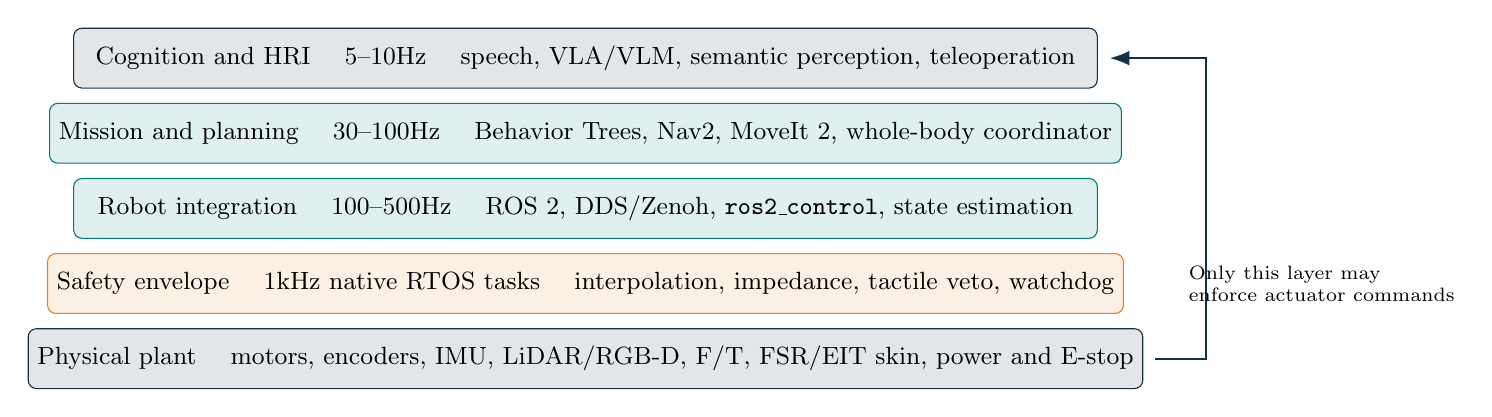
\begin{tikzpicture}[every node/.style={font=\small,align=center},layer/.style={draw=#1,fill=#1!12,rounded corners=3pt,minimum width=13.0cm,minimum height=0.76cm}]
\node[layer=navy] (cog) {Cognition and HRI \quad 5--10Hz \quad speech, VLA/VLM, semantic perception, teleoperation};
\node[layer=teal,below=0.18cm of cog] (mission) {Mission and planning \quad 30--100Hz \quad Behavior Trees, Nav2, MoveIt~2, whole-body coordinator};
\node[layer=teal,below=0.18cm of mission] (integration) {Robot integration \quad 100--500Hz \quad ROS~2, DDS/Zenoh, \texttt{ros2\_control}, state estimation};
\node[layer=orange,below=0.18cm of integration] (safety) {Safety envelope \quad 1kHz native RTOS tasks \quad interpolation, impedance, tactile veto, watchdog};
\node[layer=navy,below=0.18cm of safety] (plant) {Physical plant \quad motors, encoders, IMU, LiDAR/RGB-D, F/T, FSR/EIT skin, power and E-stop};
\draw[-{Latex[length=2.5mm]},thick,navy] ($(plant.east)+(0.15,0)$)--++(0.65,0)|-($(cog.east)+(0.15,0)$);
\node[right=0.7cm of safety,font=\scriptsize,align=left] {Only this layer may\\ enforce actuator commands};
\end{tikzpicture}
\caption{Reference multi-rate software architecture. High-level components propose intent; the safety envelope owns physical execution.}
\label{fig:multirate}
\end{figure}

\subsection{Command contract}
Every layer consumes and emits a constrained artefact: a VLA produces a proposed goal, the mission manager selects a skill, the planner produces a time-stamped trajectory, the interpolator produces bounded set-points, and the MCU produces actuator commands after safety checks. Let $\Delta\mathbf{x}_{\mathrm{AI}}$ be an AI-proposed Cartesian delta. It is admissible only after projection into the currently verified feasible set:
\begin{equation}
\mathbf{x}_{\mathrm{ref}}=\Pi_{\mathcal{F}(\mathbf{q},\mathcal{E},\mathcal{S})}\left(\mathbf{x}+\Delta\mathbf{x}_{\mathrm{AI}}\right),
\label{eq:projection}
\end{equation}
where $\mathcal{F}$ encodes joint, collision, workspace, base-stability, speed-zone and safety constraints; $\mathcal{E}$ is the current environment model; and $\mathcal{S}$ is the safety state. A rejected projection is an observable recovery event, not a silent failure.

\section{High-level software design}
\subsection{Cognition, perception and interaction}
The high-level compute domain runs on Jetson Orin AGX/Nano or an industrial GPU host. It ingests stereo/RGB-D, LiDAR, IMU, microphone and facility data. Proposed components are: Whisper-class speech-to-text; VLA/VLM models such as OpenVLA or Pi0; YOLOv11 object detection; SAM/instance segmentation; pose/scene services such as FoundationPose and nvblox/TSDF/ESDF; and a head-attention service using TDOA sound direction, gaze target and expression display. Open-vocabulary 3D grounding, panoramic perception and world-action models are candidate research modules, not safety-critical dependencies.

\begin{figure}[ht]
\centering
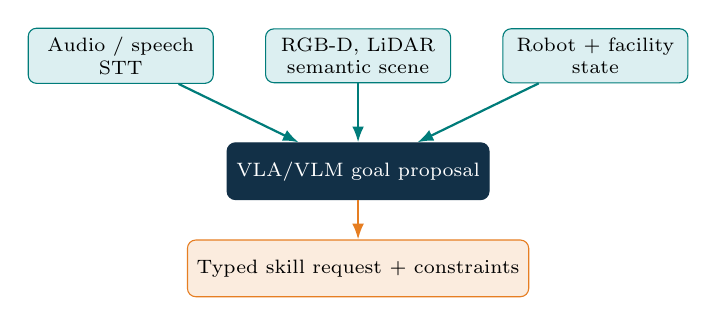
\begin{tikzpicture}[node distance=0.48cm and 0.65cm,every node/.style={font=\scriptsize,align=center},box/.style={draw=teal,fill=sky,rounded corners=3pt,minimum width=2.35cm,minimum height=0.68cm}]
\node[box] (voice) {Audio / speech\\STT};
\node[box,right=of voice] (vision) {RGB-D, LiDAR\\semantic scene};
\node[box,right=of vision] (state) {Robot + facility\\state};
\node[draw=navy,fill=navy,text=white,rounded corners=3pt,minimum width=3.0cm,minimum height=0.72cm,below=0.75cm of vision] (vla) {VLA/VLM goal proposal};
\node[draw=orange,fill=orange!15,rounded corners=3pt,minimum width=3.0cm,minimum height=0.72cm,below=0.5cm of vla] (skills) {Typed skill request + constraints};
\draw[-{Latex[length=2mm]},thick,teal] (voice)--(vla);
\draw[-{Latex[length=2mm]},thick,teal] (vision)--(vla);
\draw[-{Latex[length=2mm]},thick,teal] (state)--(vla);
\draw[-{Latex[length=2mm]},thick,orange] (vla)--(skills);
\end{tikzpicture}
\caption{Cognitive data flow. The only output to autonomy is a typed, constrained skill request.}
\label{fig:cognition}
\end{figure}

\subsection{Mission orchestration and recoverable skills}
Use BehaviorTree.CPP as the mission-control surface, with explicit lifecycle and recovery nodes. A top-level tree should sequence \texttt{AcquireGoal}, \texttt{ValidateContext}, \texttt{Navigate}, \texttt{Observe}, \texttt{Manipulate}, \texttt{Verify}, \texttt{Deliver} and \texttt{Report}. Each action has timeout, cancellation, degraded-mode and recovery semantics. Required bimanual recovery nodes include object slip, grasp failure, base obstruction, unreachable pose, perception loss, communication loss, door/elevator failure and operator handover.

\begin{table}[ht]
\centering\small
\caption{Representative high-level skills and their required guards.}
\begin{tabularx}{\textwidth}{@{}lYY@{}}
\toprule
Skill & Planner / service composition & Preconditions and verification \\
\midrule
Navigate to workstation & Nav2 SLAM, costmaps, MPPI/DWB, speed zones & Localisation valid; footprint free; arrival tolerance met \\
Pick / place & Perception, MoveIt~2, grasp planner, tactile close & Object confidence; collision-free plan; grasp/contact verification \\
Bimanual carry / handover & Whole-body coordinator, dual-arm plans, base motion & Object constraint; synchronisation; human/obstacle clearance \\
Door / elevator routine & Guarded force motion, perception, building/WMS interface & Access granted; force limit; fallback/operator request \\
Charge / dock & Nav2 docking, BMS and charging-contact service & Battery threshold; charger detection; current/thermal checks \\
\bottomrule
\end{tabularx}
\end{table}

\subsection{Navigation, manipulation and whole-body coordination}
Nav2 owns localisation, global route generation, local obstacle avoidance and speed-zone compliance. MoveIt~2 owns arm kinematics, collision checking and trajectory generation. \texttt{ros2\_control} owns controller lifecycle and command transport. For mobile manipulation, the base and lift must appear in the robot model, even when coarse base positioning is scheduled separately. A whole-body coordinator resolves the common stop-then-move failure mode by choosing whether base, lift and arms may move concurrently; it may use model-predictive or SDF-based optimisation where validated.\cite{bonci,liwb}

\subsection{Middleware and QoS}
ROS~2 Jazzy/Humble is the integration backbone. DDS remains a suitable default for discovery and QoS; \texttt{rmw\_zenoh} is a candidate transport where shared-memory local IPC or constrained wireless links justify it. QoS policy is data-class specific: high-rate images/point clouds use best-effort, bounded queues and freshness constraints; joint state, action results, safety state and configuration use reliable delivery with explicit deadlines/liveliness. The safety loop must not rely on DDS delivery to stop a robot.

\section{Low-level software design}
\subsection{Hardware abstraction and fieldbus topology}
The low-level architecture is divided between a Linux-side \texttt{ros2\_control} hardware interface and native MCU firmware. EtherCAT is recommended for high-axis-count, synchronised servo configurations; CAN-FD/CANopen is an appropriate cost-sensitive distributed-control alternative. The project synthesis identifies VESC/ODrive BLDC controllers, dual STM32H7/ESP32 microcontrollers and dirty 24--48V versus isolated clean 12/19V domains. This maps to a hardware inventory service that exposes serial number, firmware revision, calibration, fault state and power-domain diagnostics for every module.

\begin{figure}[ht]
\centering
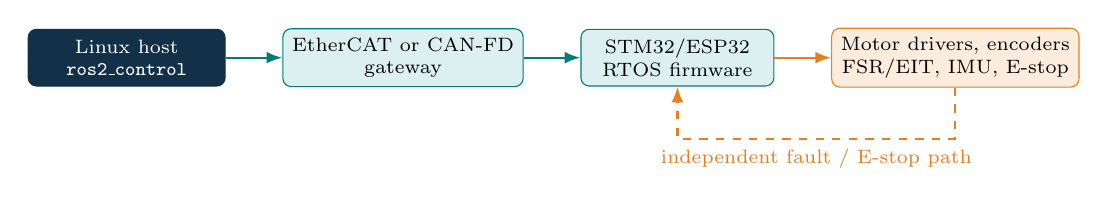
\begin{tikzpicture}[node distance=0.55cm and 0.72cm,every node/.style={font=\scriptsize,align=center},box/.style={draw=teal,fill=sky,rounded corners=3pt,minimum width=2.45cm,minimum height=0.72cm}]
\node[draw=navy,fill=navy,text=white,rounded corners=3pt,minimum width=2.5cm,minimum height=0.72cm] (host) {Linux host\\\texttt{ros2\_control}};
\node[box,right=of host] (gateway) {EtherCAT or CAN-FD\\gateway};
\node[box,right=of gateway] (mcu) {STM32/ESP32\\RTOS firmware};
\node[draw=orange,fill=orange!15,rounded corners=3pt,minimum width=2.6cm,minimum height=0.72cm,right=of mcu] (motor) {Motor drivers, encoders\\FSR/EIT, IMU, E-stop};
\draw[-{Latex[length=2mm]},thick,teal] (host)--(gateway);
\draw[-{Latex[length=2mm]},thick,teal] (gateway)--(mcu);
\draw[-{Latex[length=2mm]},thick,orange] (mcu)--(motor);
\draw[-{Latex[length=2mm]},dashed,thick,orange] (motor.south)--++(0,-0.65)-|node[pos=0.25,below,font=\scriptsize]{independent fault / E-stop path}(mcu.south);
\end{tikzpicture}
\caption{Control-path ownership. ROS~2 requests motion; native firmware enforces timing and physical limits.}
\label{fig:lowlevel}
\end{figure}

\subsection{Native real-time firmware}
The MCU executes FreeRTOS, Zephyr or a carefully bounded bare-metal schedule. The 1kHz motor/impedance task runs natively and must be decoupled from micro-ROS callback handling; micro-ROS is an asynchronous telemetry, parameter and command bridge. A representative scheduling design is: (i) highest priority: hardware E-stop, current/overtemperature and deadline monitor; (ii) 1kHz: encoder acquisition, FOC/servo update, impedance/tactile filter and actuator limit; (iii) lower priority: fieldbus RX/TX; (iv) lowest priority: micro-ROS, logs and calibration requests.

\subsection{Trajectory interpolation and contact control}
High-level deltas at 5--10Hz cannot drive motors directly. A trajectory service converts accepted goals into bounded, time-stamped reference segments; a cubic spline or jerk-limited generator produces $q_d(t)$ and $\dot q_d(t)$. The local controller calculates
\begin{equation}
\tau_{\mathrm{cmd}}=K_p(q_d-q)+K_d(\dot q_d-\dot q)+\tau_{\mathrm{ff}},
\qquad
\mathbf{F}_{\mathrm{cmd}}=\mathbf{K}(\mathbf{x}_d-\mathbf{x})+\mathbf{D}(\dot{\mathbf{x}}_d-\dot{\mathbf{x}}).
\label{eq:impedance}
\end{equation}
The MCU clamps torque, velocity and power; when tactile, F/T or EIT contact is above a configured envelope, it reduces stiffness, freezes/retreats according to the skill policy, and reports a safety event. The supplied sources cite a 25N threshold for one tactile-veto proposal; the deployed threshold must be risk-assessed for the specific hand, task and standard.

\subsection{Safety state machine}
\begin{figure}[ht]
\centering
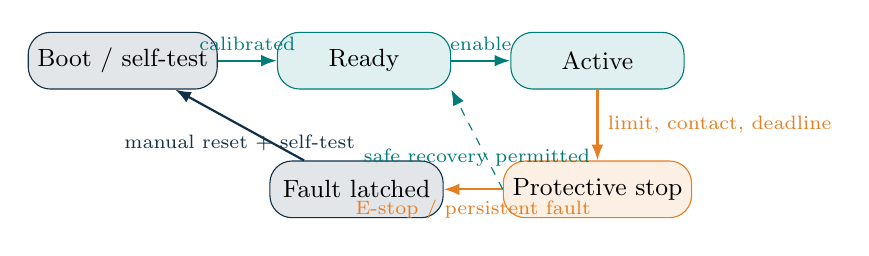
\begin{tikzpicture}[node distance=0.75cm and 0.75cm,every node/.style={font=\small,align=center},state/.style={draw=#1,fill=#1!12,rounded corners=8pt,minimum width=2.2cm,minimum height=0.72cm}]
\node[state=navy] (boot) {Boot / self-test};
\node[state=teal,right=of boot] (ready) {Ready};
\node[state=teal,right=of ready] (active) {Active};
\node[state=orange,below=0.9cm of active] (protect) {Protective stop};
\node[state=navy,left=of protect] (fault) {Fault latched};
\draw[-{Latex[length=2mm]},thick,teal] (boot)--node[above,font=\scriptsize]{calibrated} (ready);
\draw[-{Latex[length=2mm]},thick,teal] (ready)--node[above,font=\scriptsize]{enable} (active);
\draw[-{Latex[length=2mm]},thick,orange] (active)--node[right,font=\scriptsize]{limit, contact, deadline} (protect);
\draw[-{Latex[length=2mm]},thick,orange] (protect)--node[below,font=\scriptsize]{E-stop / persistent fault} (fault);
\draw[-{Latex[length=2mm]},thick,navy] (fault)--node[below,font=\scriptsize]{manual reset + self-test} (boot);
\draw[-{Latex[length=2mm]},dashed,teal] (protect.west)--node[below,font=\scriptsize]{safe recovery permitted} (ready.south east);
\end{tikzpicture}
\caption{Safety states. The exact transition conditions require a hazard analysis and hardware implementation; no software-only state is accepted as an E-stop substitute.}
\label{fig:safety}
\end{figure}

\section{Digital twin, data and deployment operations}
\subsection{Simulation and sim-to-real}
Isaac Sim/Isaac Lab with OpenUSD is recommended for sensor twins, synthetic data, scalable policy training and SIL/vHIL workflows. MuJoCo provides a complementary environment for contact-rich and tendon-driven studies; Gazebo remains a useful open Nav2/MoveIt integration baseline. The promotion sequence is Model-in-the-Loop $\rightarrow$ SIL $\rightarrow$ vHIL $\rightarrow$ supervised hardware $\rightarrow$ bounded autonomous deployment. Domain randomisation covers lighting, textures, sensor noise/latency, mass, friction, wheel slip and selected contact parameters.\cite{isaac,isaaclab,mujoco,gazebo}

\subsection{Data products and teleoperation}
VR/web teleoperation provides demonstrations and operator assistance. Every episode should synchronise sensor data, robot state, command state, safety events, calibration versions and environment/task labels. Store raw data separately from curated training datasets; record consent, retention and access controls where people appear in audio/video. Dataset quality should be measured by task coverage, intervention count, distribution shift and replay success---not only episode count.

\subsection{Containerised releases, OTA and fleet services}
The market analysis identifies software/services, OTA and fleet operations as a major value layer. Package high-level applications in tested OCI/Docker images, with immutable release manifests covering ROS distribution, CUDA/TensorRT, model version, map/skill set and configuration schema. The safety firmware has a separately controlled, signed update path. Fleet updates are staged: simulation, bench hardware, canary robot, limited fleet and broad fleet; every phase has health gates and rollback. WMS/ERP/IoT integration should be asynchronous and unable to command motion directly.

\begin{figure}[ht]
\centering
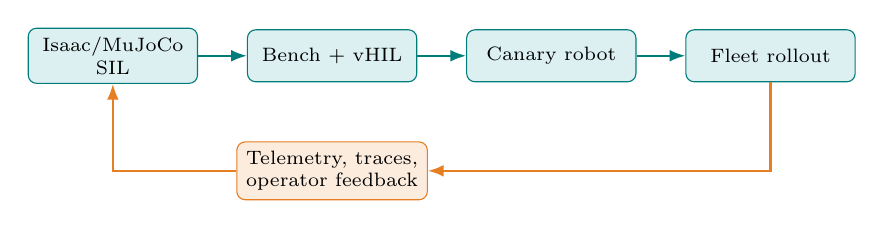
\begin{tikzpicture}[node distance=0.48cm and 0.62cm,every node/.style={font=\scriptsize,align=center},box/.style={draw=teal,fill=sky,rounded corners=3pt,minimum width=2.15cm,minimum height=0.66cm}]
\node[box] (sim) {Isaac/MuJoCo\\SIL};
\node[box,right=of sim] (bench) {Bench + vHIL};
\node[box,right=of bench] (canary) {Canary robot};
\node[box,right=of canary] (fleet) {Fleet rollout};
\node[draw=orange,fill=orange!15,rounded corners=3pt,minimum width=2.2cm,minimum height=0.66cm,below=0.75cm of bench] (telemetry) {Telemetry, traces,\\ operator feedback};
\draw[-{Latex[length=2mm]},thick,teal] (sim)--(bench);
\draw[-{Latex[length=2mm]},thick,teal] (bench)--(canary);
\draw[-{Latex[length=2mm]},thick,teal] (canary)--(fleet);
\draw[-{Latex[length=2mm]},thick,orange] (fleet.south)|-(telemetry.east);
\draw[-{Latex[length=2mm]},thick,orange] (telemetry.west)-|(sim.south);
\end{tikzpicture}
\caption{Release and learning lifecycle. Health gates, observability and rollback are part of the runtime design.}
\label{fig:release}
\end{figure}

\section{Interfaces, packages and verification plan}
\subsection{Recommended package boundaries}
\begin{longtable}{@{}p{0.22\textwidth}p{0.32\textwidth}p{0.36\textwidth}@{}}
\caption{Package-level ownership and interfaces.}\\
\toprule
Package / domain & Responsibilities & Contract / verification \\
\midrule
\endfirsthead
\toprule Package / domain & Responsibilities & Contract / verification \\
\midrule\endhead
\texttt{robot\_description} & URDF/Xacro, SRDF, TF frames, collision geometry, limits & Versioned model; CI validates transforms, joint limits and collision pairs \\
\texttt{perception\_stack} & Sensor drivers, calibration, detection, segmentation, pose and scene map & Timestamp/frame convention, confidence and freshness fields \\
\texttt{mission\_bt} & Typed goal acceptance, skill sequencing, recovery and operator escalation & Deterministic tree tests, timeout/cancellation coverage \\
\texttt{navigation\_stack} & SLAM, localisation, Nav2, docking, costmaps and speed zones & Map/version identity, localisation covariance, safety-zone API \\
\texttt{manipulation\_stack} & MoveIt~2, grasping, whole-body coordination, guarded motion & Time-stamped trajectory, constraints and verification event \\
\texttt{control\_bridge} & \texttt{ros2\_control} hardware interface, state/command conversion & Controller lifecycle; command saturation and stale-command tests \\
\texttt{mcu\_firmware} & RTOS tasks, servo/FOC, tactile safety, watchdog, fieldbus & WCET, jitter, fault and E-stop test traces \\
\texttt{fleet\_ops} & OTA, telemetry, device inventory, release gates, WMS adapters & Signed manifests, audit record, rollback and access-control tests \\
\bottomrule
\end{longtable}

\subsection{Verification matrix}
\begin{table}[ht]
\centering\small
\begin{tabularx}{\textwidth}{@{}lYY@{}}
\toprule
Test stage & What is tested & Exit criterion \\
\midrule
Unit / static analysis & Schema, kinematics, command limits, controller logic, firmware memory safety & All safety-relevant paths reviewed and tested \\
Simulation / SIL & Planning, perception, task trees, domain randomisation, failure injection & Defined success and no unhandled safety transitions \\
Bench / vHIL & Fieldbus, timing, actuator emulator, tactile inputs, power transients & Measured timing budget and safe response to injected faults \\
Supervised hardware & Calibrated robot, guarded motion, E-stop, recovery & Safety-state traces and task-level acceptance metrics \\
Pilot / fleet & OTA, WMS integration, observability, uptime and intervention rate & Canary health gate, rollback demonstrated \\
\bottomrule
\end{tabularx}
\end{table}

\section{Implementation roadmap}
\textbf{Phase 1---Safe platform baseline.} Establish robot model, hardware inventory, sensor drivers, \texttt{ros2\_control}, native 1kHz firmware, E-stop, diagnostics and simulation. No VLA is required.

\textbf{Phase 2---Bounded autonomy.} Add Nav2, MoveIt~2, behavior-tree missions, guarded grasps, docking and teleoperation. Validate recovery and hardware-in-the-loop tests.

\textbf{Phase 3---Cognitive assistance.} Introduce speech, semantic perception and VLA-proposed skill parameters behind typed goal validation and operator supervision.

\textbf{Phase 4---Fleet productisation.} Add container release management, signed OTA, WMS/IoT connectors, telemetry dashboards and data governance. Measure deployment effort, availability and intervention rate.

\section{Conclusion}
The recommended software design makes autonomy useful without making it the only line of defence. ROS~2, Nav2, MoveIt~2 and \texttt{ros2\_control} supply a modular high- and mid-level foundation; RTOS-native firmware, fieldbus discipline and independent safety state transitions own physical execution; Isaac/OpenUSD and teleoperation support iteration; and fleet operations turn the robot into a maintainable product. This is the appropriate architecture for a semi-humanoid system whose novelty lies in dependable, modular integration across cognition, manipulation and safe real-world operation.

\begin{thebibliography}{99}\small
\bibitem{bonci} A. Bonci, F. Gaudeni, and M. Giannini, ``ROS2-Based Frameworks for Increasing Robot Autonomy: A Survey,'' \emph{Applied Sciences}, 2023. DOI: \url{https://doi.org/10.3390/app132312796}.
\bibitem{liwb} Y. Li, L. Yin, and T. Zhang, ``Real-time Whole-Body Motion Planning for Mobile Manipulators Carrying Arbitrarily Shaped Payloads via Kinematically-Coupled SVSDF,'' arXiv:2608.07005, 2026. \url{https://arxiv.org/abs/2608.07005}.
\bibitem{isaac} NVIDIA, ``Isaac AI Robot Development Platform,'' \url{https://developer.nvidia.com/isaac}.
\bibitem{isaaclab} M. Mittal et al., ``Isaac Lab: High-Performance Robot Learning Framework Built on NVIDIA Isaac Sim,'' arXiv:2403.07257, 2024. \url{https://arxiv.org/abs/2403.07257}.
\bibitem{mujoco} DeepMind, ``MuJoCo,'' \url{https://mujoco.org/}.
\bibitem{gazebo} Open Robotics, ``Gazebo,'' \url{https://gazebosim.org/}.
\bibitem{iovino} M. Iovino et al., ``A Survey of Behavior Trees in Robotics and AI,'' \emph{Robotics and Autonomous Systems}, 2022. DOI: \url{https://doi.org/10.1016/j.robot.2022.104096}.
\bibitem{openvla} M. J. Kim et al., ``OpenVLA: An Open-Source Vision-Language-Action Model,'' arXiv:2406.09246, 2024. \url{https://arxiv.org/abs/2406.09246}.
\bibitem{micro} N. Stoufs et al., ``Budget-Based Real-Time Executor for Micro-ROS,'' arXiv:2105.05590, 2021. \url{https://arxiv.org/abs/2105.05590}.
\end{thebibliography}
\end{document}
